%%%%%%%%%%%%%%%%%%%%%%%%%%%%%%%%%%%%%%%%%
% Beamer Presentation
% LaTeX Template
% Version 1.0 (10/11/12)
%
% This template has been downloaded from:
% http://www.LaTeXTemplates.com
%
% License:
% CC BY-NC-SA 3.0 (http://creativecommons.org/licenses/by-nc-sa/3.0/)
%
%%%%%%%%%%%%%%%%%%%%%%%%%%%%%%%%%%%%%%%%%

%----------------------------------------------------------------------------------------
%	PACKAGES AND THEMES
%----------------------------------------------------------------------------------------

\documentclass{beamer}

\mode<presentation> {

% The Beamer class comes with a number of default slide themes
% which change the colors and layouts of slides. Below this is a list
% of all the themes, uncomment each in turn to see what they look like.

%\usetheme{default}
%\usetheme{AnnArbor}
%\usetheme{Antibes}
%\usetheme{Bergen}
%\usetheme{Berkeley}
%\usetheme{Berlin}
%\usetheme{Boadilla}
%\usetheme{CambridgeUS}
%\usetheme{Copenhagen}
%\usetheme{Darmstadt}
%\usetheme{Dresden}
%\usetheme{Frankfurt}
%\usetheme{Goettingen}
%\usetheme{Hannover}
%\usetheme{Ilmenau}
%\usetheme{JuanLesPins}
%\usetheme{Luebeck}
\usetheme{Madrid}
%\usetheme{Malmoe}
%\usetheme{Marburg}
%\usetheme{Montpellier}
%\usetheme{PaloAlto}
%\usetheme{Pittsburgh}
%\usetheme{Rochester}
%\usetheme{Singapore}
\usetheme{Szeged}
%\usetheme{Warsaw}

% As well as themes, the Beamer class has a number of color themes
% for any slide theme. Uncomment each of these in turn to see how it
% changes the colors of your current slide theme.

%\usecolortheme{albatross}
%\usecolortheme{beaver}
%\usecolortheme{beetle}
%\usecolortheme{crane}
%\usecolortheme{dolphin}
%\usecolortheme{dove}
%\usecolortheme{fly}
%\usecolortheme{lily}
%\usecolortheme{orchid}
%\usecolortheme{rose}
%\usecolortheme{seagull}
%\usecolortheme{seahorse}
%\usecolortheme{whale}
%\usecolortheme{wolverine}

%\setbeamertemplate{footline} % To remove the footer line in all slides uncomment this line
%\setbeamertemplate{footline}[page number] % To replace the footer line in all slides with a simple slide count uncomment this line

\setbeamertemplate{navigation symbols}{} % To remove the navigation symbols from the bottom of all slides uncomment this line
}

\usepackage{verbatim}
\usepackage{graphicx} % Allows including images
\usepackage{booktabs} % Allows the use of \toprule, \midrule and \bottomrule in tables

%----------------------------------------------------------------------------------------
%	TITLE PAGE
%----------------------------------------------------------------------------------------

\title[PMAAS]{Performance Modeling as a Service} % The short title appears at the bottom of every slide, the full title is only on the title page

\author{Mark Meredith} % Your name
\institute[Penn State] % Your institution as it will appear on the bottom of every slide, may be shorthand to save space
{
Pennsylvania State University \\ % Your institution for the title page
\medskip
\textit{mwm126@cse.psu.edu} % Your email address
}
\date{\today} % Date, can be changed to a custom date

\begin{document}

\begin{frame}
\titlepage % Print the title page as the first slide
\end{frame}

\begin{frame}
\frametitle{Overview} % Table of contents slide, comment this block out to remove it
\tableofcontents % Throughout your presentation, if you choose to use \section{} and \subsection{} commands, these will automatically be printed on this slide as an overview of your presentation
\end{frame}

%----------------------------------------------------------------------------------------
%	PRESENTATION SLIDES
%----------------------------------------------------------------------------------------

%------------------------------------------------
%\section{Introduction} % Sections can be created in order to organize your presentation into discrete blocks, all sections and subsections are automatically printed in the table of contents as an overview of the talk
%\------------------------------------------------

%\subsection{Subsection Example} % A subsection can be created just before a set of slides with a common theme to further break down your presentation into chunks

\section{Background}
\begin{frame}
\frametitle{Lots of VMs from cloud vendors...}
\begin{figure}[htbp]
\centering
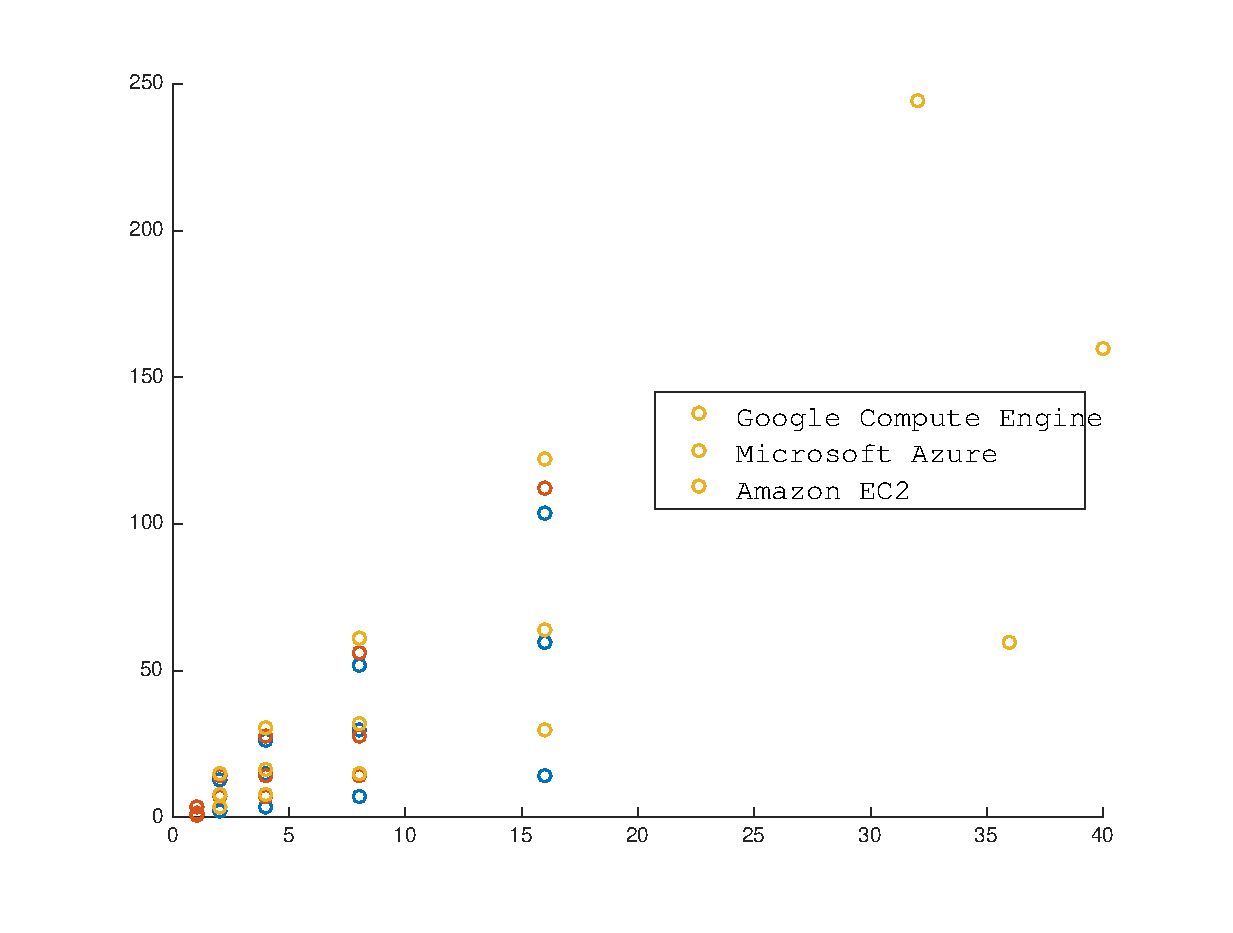
\includegraphics[width=0.45\textwidth]{cloud_vm_types.eps}
\end{figure}
\end{frame}

\begin{frame}
\frametitle{How to estimate performance?}
\begin{figure}[htbp]
\centering
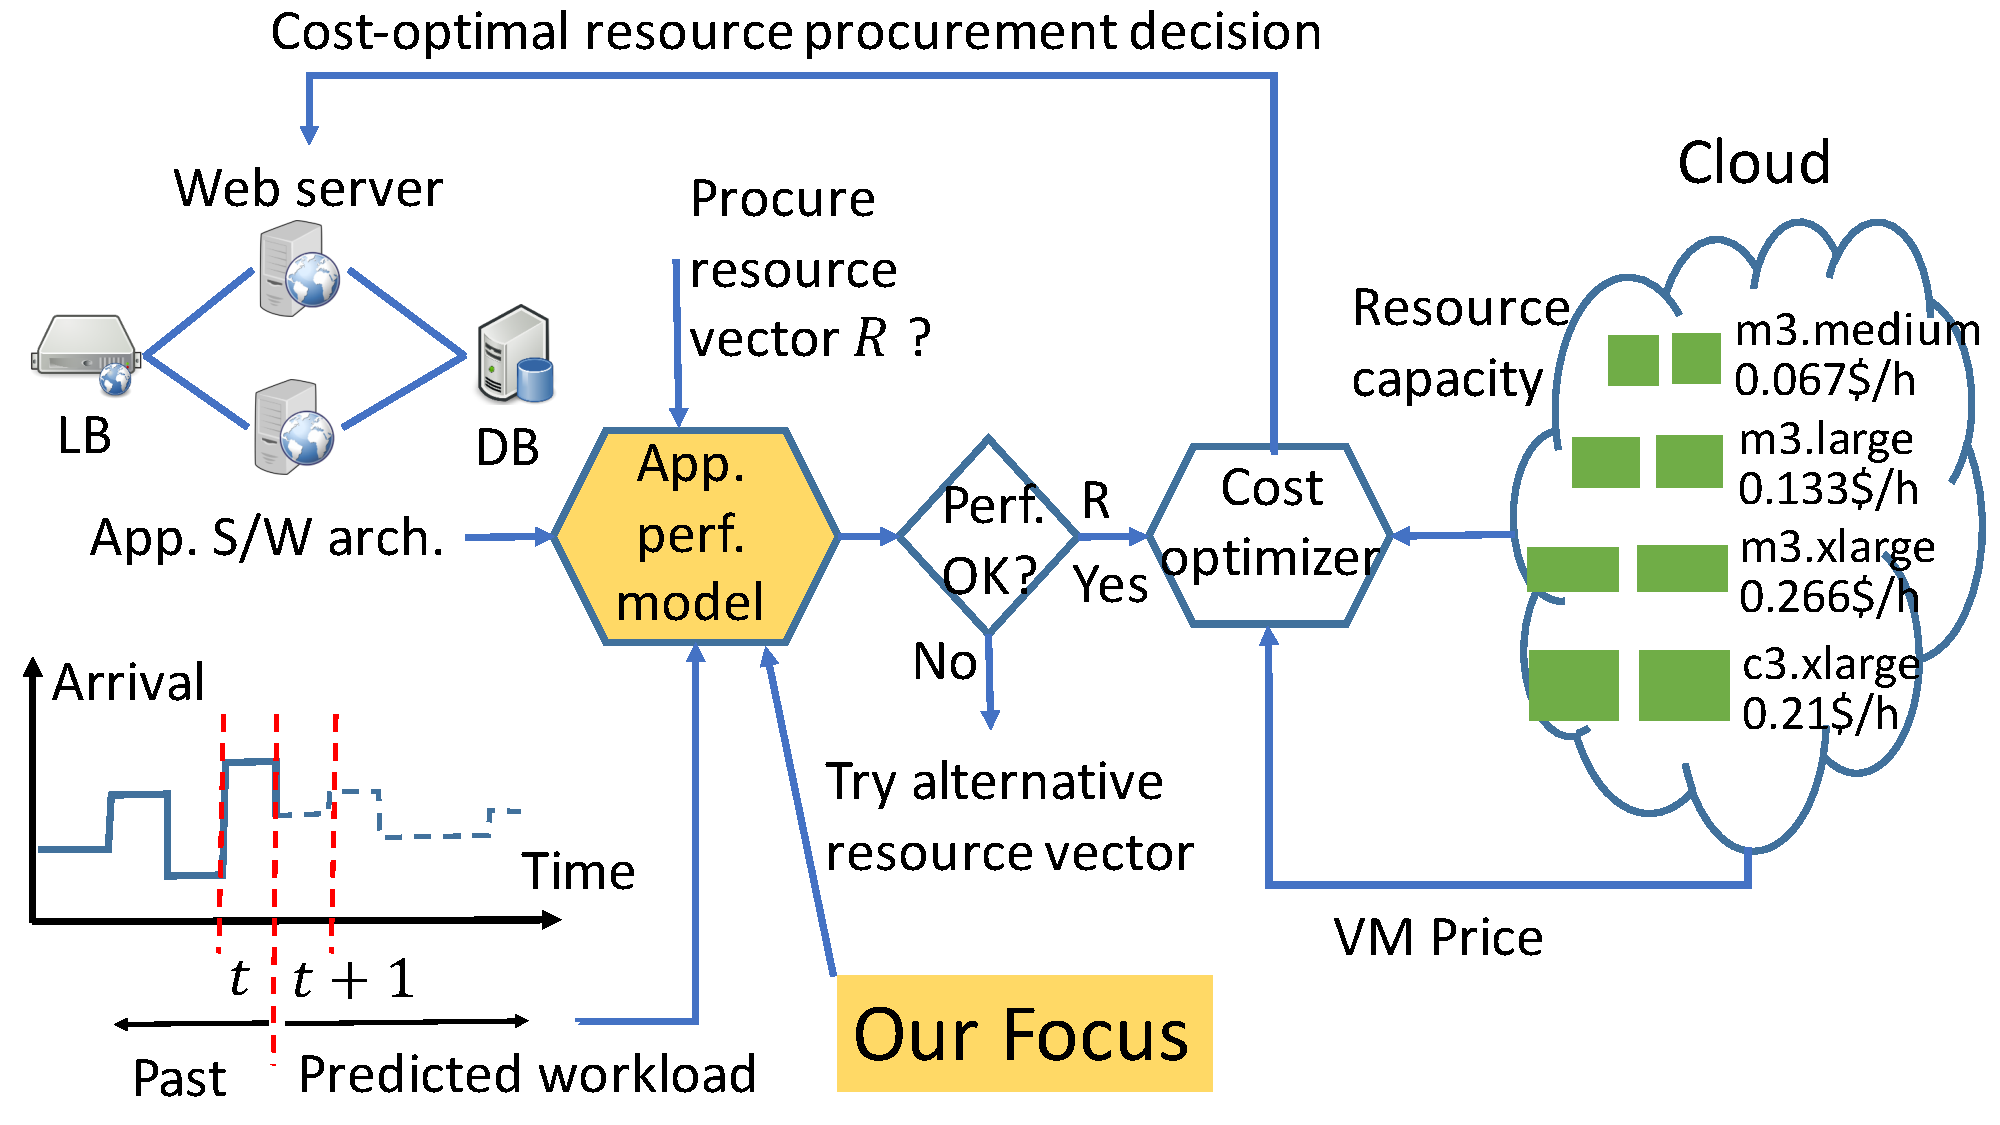
\includegraphics[width=0.8\textwidth]{system}
\end{figure}
\end{frame}

\begin{frame}
\frametitle{Black box Modeling}
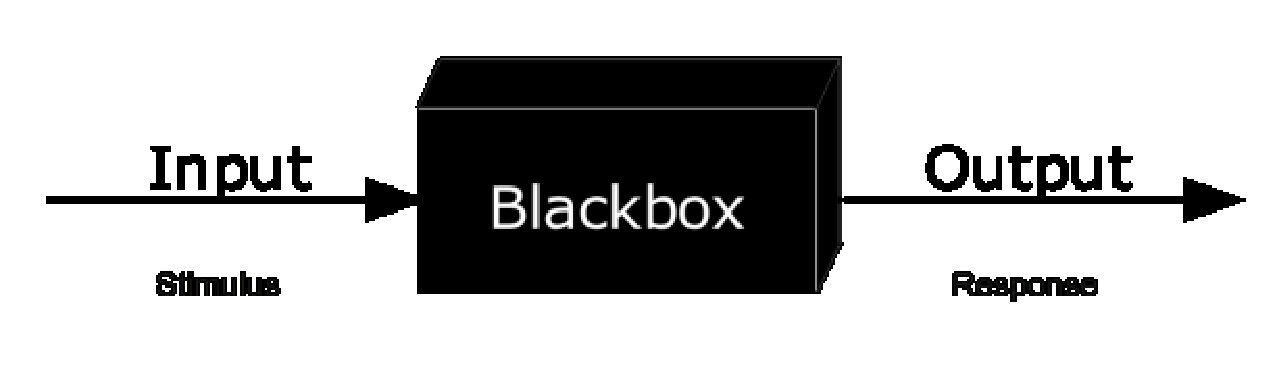
\includegraphics[width=0.8\textwidth]{blackbox.eps}
\end{frame}

\begin{frame}
\frametitle{Latency vs Throughput}
\begin{block}{Nonlinear in general}
Gradual change at low throughput, rapid increase near system capacity 
\end{block}
\begin{figure}
    \centering
    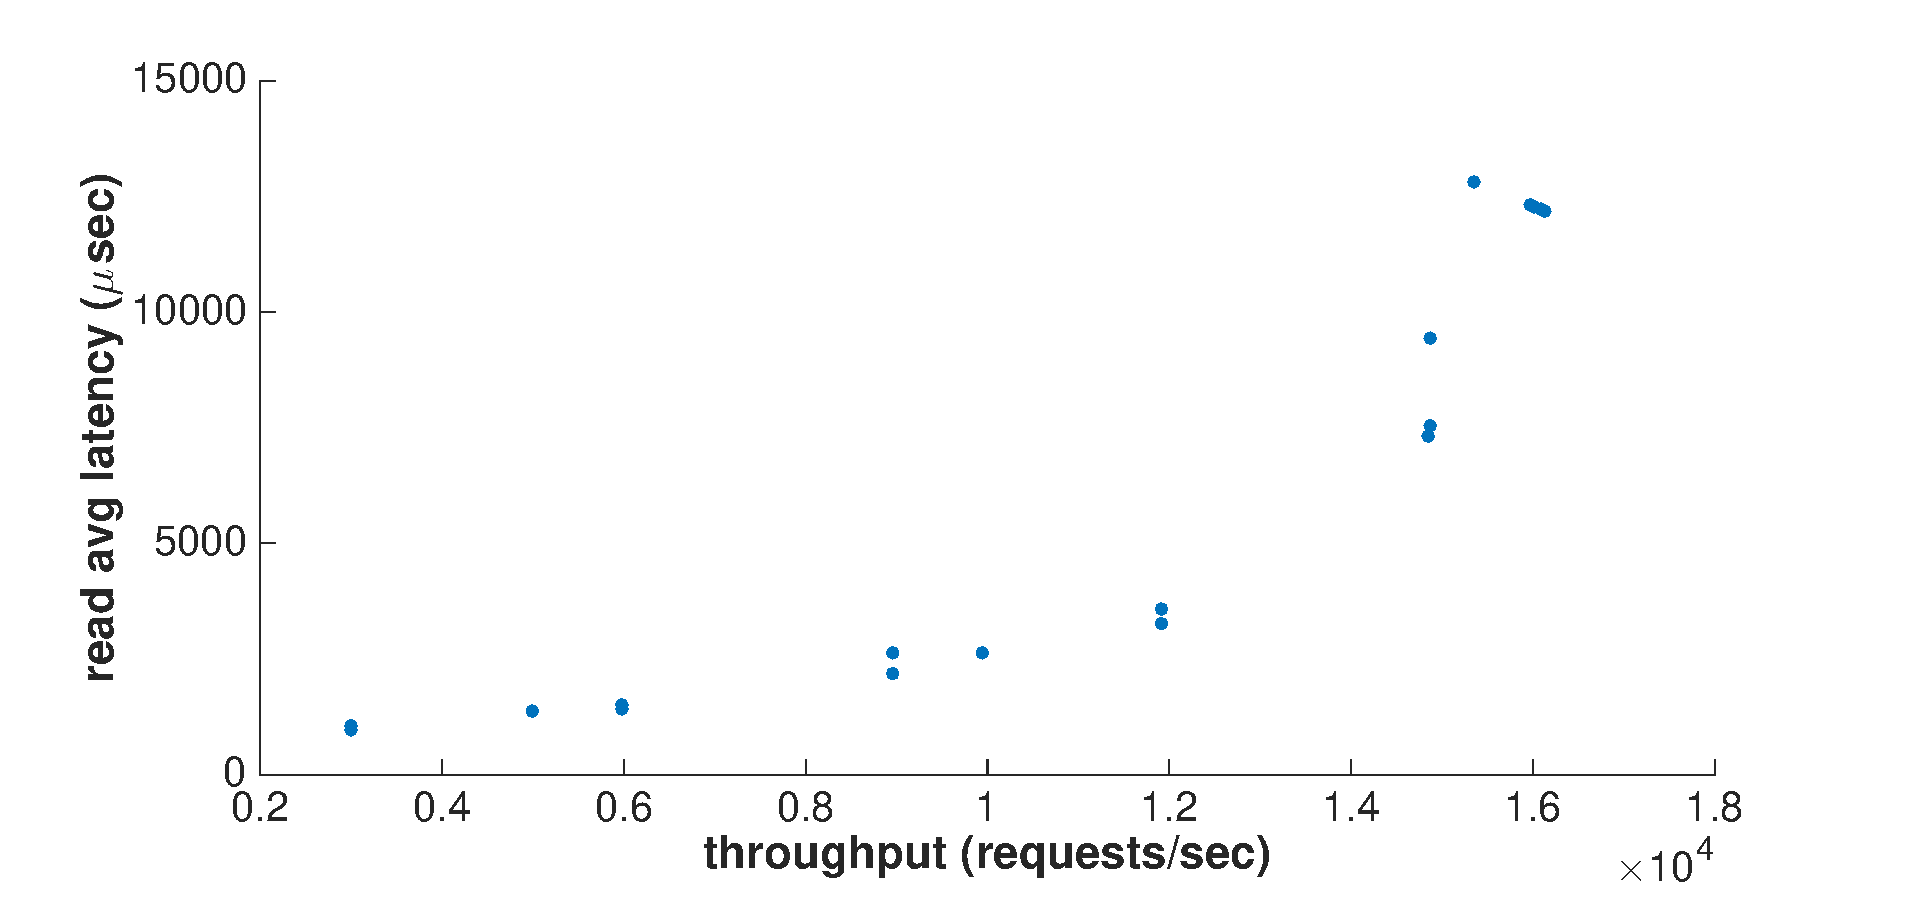
\includegraphics[scale = 0.35]{two_regions_bare.eps}
\end{figure}
\end{frame}
\begin{frame}
\frametitle{Latency vs Throughput}
\begin{block}{Focus on low-throughput region}
Linear relationship between latency and throughput
\end{block}
\begin{figure}
    \centering
    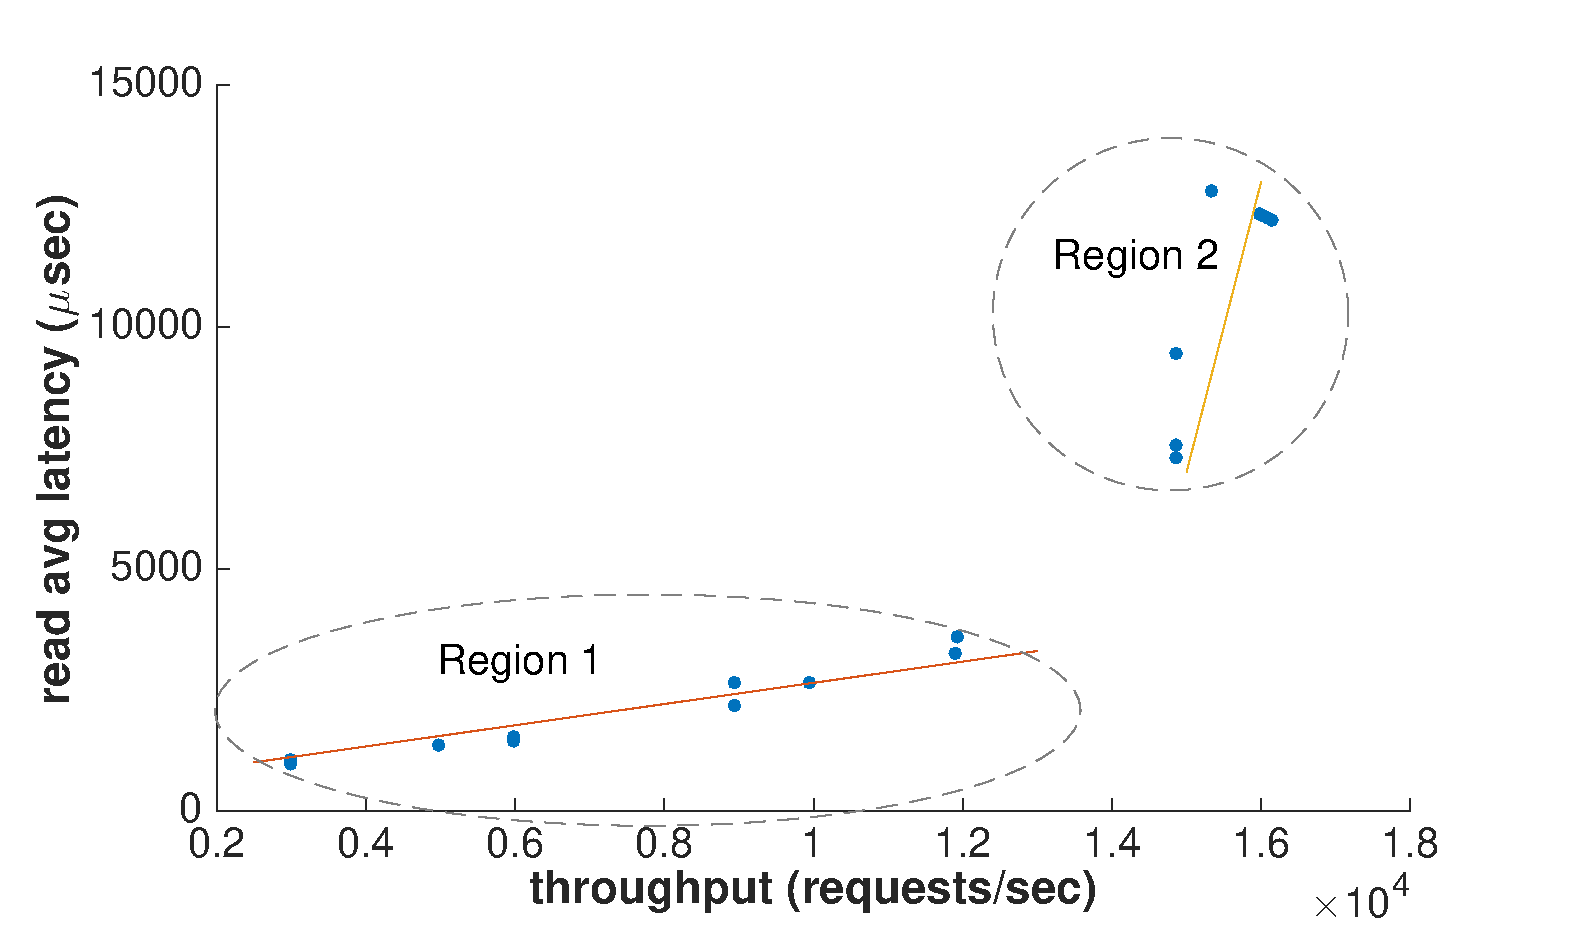
\includegraphics[scale = 0.35]{two_regions.eps}
\end{figure}
\end{frame}

\section{Model}
\begin{frame}
\frametitle{Multiple Linear Regression}
Dependent variable $y$, independent variables $x_1,\ldots,x_p$
\begin{displaymath}{
y_i = \beta_1 x_{i1}+\ldots+\beta_{p}x_{ip}+\epsilon_i
}\end{displaymath}

Do a multiple linear regression to find the coefficients $\beta_i$.  Then for a test instance $VM_{test}$ with $x_{test,i}$, find:
\begin{displaymath}{
y_{test} = \beta_1 x_{test,1}+\ldots+\beta_{p}x_{test,p}+\epsilon_i = \hat{y}+\epsilon_i 
}\end{displaymath}

\end{frame}

\begin{frame}
\frametitle{Multiple Linear Regression}
Predicted coefficient of determination:
\begin{displaymath}
R_{predicted}^2=1-\frac{\sum_{i=1}^{n} (y_{test,i} - \hat{y}(x_{test,i}))^{2}}{\sum_{i=1}^{n} (y_{test,i} - \bar{y_{test}})^{2}}
\end{displaymath}
where
\begin{displaymath}
\hat{y}(x_{test})=\sum_{i=1}^{n} \beta_i x_{test,i}
\qquad\text{and}\qquad
\bar{y}_{test}=\frac{1}{n}\sum_{i=1}^{n} y_{test,i}
\end{displaymath}
\end{frame}
\section{Testing}

\begin{frame}
\frametitle{Databases used in testing}
\begin{block}{Redis}
Most popular Key-value database
\end{block}
\begin{block}{Apache Cassandra}
Most scalable NoSQL database
\end{block}
\begin{block}{MySQL}
Most widely used open-source RDBMS
\end{block}
\end{frame}

\begin{frame}
\frametitle{Benchmark specifics}
\begin{itemize}
\item Yahoo! Cloud Serving Benchmark 
\item ran YCSB client on m4.2xlarge EC2 instance with Ubuntu Linux 14.04
\begin{itemize}
\item checked client system load to make sure client is not the bottleneck
\end{itemize}
\item tested from same Amazon zone/region
\item preloaded database before each test with a million records each with 10 fields of size 100 bytes of data
\item ran benchmark for a million requests
\end{itemize}
\end{frame}

\begin{frame}
\frametitle{Benchmark specifics}
AWS instances used in testing:
\begin{table}
\begin{tabular}{|r|l|c|r|l|} \hline
Instance name & Abbr.& \# cores&Memory&Network\\ \hline
m3.large & $VM_1$ & 2 & 7.5 GB & Moderate\\ \hline
m3.xlarge & $VM_2$ & 4 & 15 GB & Moderate\\ \hline
m3.2xlarge & $VM_3$ & 8 & 30 GB & High\\ \hline
r3.large & $VM_4$ & 2 & 15 GB & Moderate\\ \hline
r3.xlarge & $VM_5$ & 4 & 30.5 GB & Moderate\\ \hline
r3.2xlarge & $VM_6$ & 8 & 61 GB & High\\ \hline
\hline\end{tabular}
\end{table}
\end{frame}

\section{Results}

\begin{frame}
\frametitle{Redis}
\begin{enumerate}
\item key/value NoSQL database
\item deployed with Amazon ElastiCache
\item only used one read replica
\end{enumerate}
\end{frame}

\begin{frame}
\frametitle{Redis}
\begin{table}
\centering
\caption{Redis Latency $R_{predicted}^2$ for $VM_2$}
\begin{tabular}{|r|r|l|} \hline
read&write&Training Set\\ \hline
-0.648416 & -1.12245  & $\{VM6\}$ \\ \hline 
0.51488 &  0.41527 & $\{VM6,VM5\}$ \\ \hline 
0.738979 &  0.738969 & $\{VM6,VM3,VM5\}$ \\ \hline 
0.776002 & 0.756578  & $\{VM6,VM3,VM5,VM4\}$ \\ \hline 
0.837957 &  0.827944 & $\{VM6,VM3,VM5,VM4,VM1\}$ \\ \hline 
\hline\end{tabular}

% \centering
% \caption{Redis $R_{predicted}^2$ for $VM_2$}
% \begin{tabular}{|r|r|l|} \hline
% reads&writes&Training Set\\ \hline
% -0.648416 & -1.12245  & VM6 \\ \hline 
% 0.51488 &  0.547705 & VM6 VM5 \\ \hline 
% 0.738979 & 0.738969  & VM6 VM5 VM3 \\ \hline 
% 0.832156 &  0.756578 & VM6 VM5 VM3 VM1 \\ \hline 
% 0.837957 & 0.827944  & VM6 VM5 VM3 VM1 VM4 \\ \hline 
% \hline\end{tabular}
%\end{minipage}
% \begin{minipage}[b]{0.25\linewidth}
% \centering
% \caption{Redis $R_{predicted}^2$ for $VM_2$}
% \begin{tabular}{|r|r|l|} \hline
% reads&writes&Training Set\\ \hline
% -0.559516 & -0.47657  & VM5 \\ \hline 
% 0.260701 &  0.29636 & VM5 VM3 \\ \hline 
% 0.738979 &  0.738969 & VM5 VM3 VM6 \\ \hline 
% 0.776002 & 0.756578  & VM5 VM3 VM6 VM4 \\ \hline 
% 0.837957 & 0.827944  & VM5 VM3 VM6 VM4 VM1 \\ \hline 
% \hline\end{tabular}

% \centering
% \caption{Redis $R_{predicted}^2$ for $VM_2$}
% \begin{tabular}{|r|r|l|} \hline
% reads&writes&Training Set\\ \hline
% -0.559516 & -0.47657  & VM5 \\ \hline 
% 0.51488 & 0.547705  & VM5 VM6 \\ \hline 
% 0.738979 & 0.738969  & VM5 VM6 VM3 \\ \hline 
% 0.776002 & 0.756578  & VM5 VM6 VM3 VM4 \\ \hline 
% 0.837957 & 0.827944  & VM5 VM6 VM3 VM4 VM1 \\ \hline 
% \hline\end{tabular}
% \end{minipage}
\end{table}
\end{frame}

\begin{frame}
\frametitle{Redis}
  \begin{figure}
    \centering
    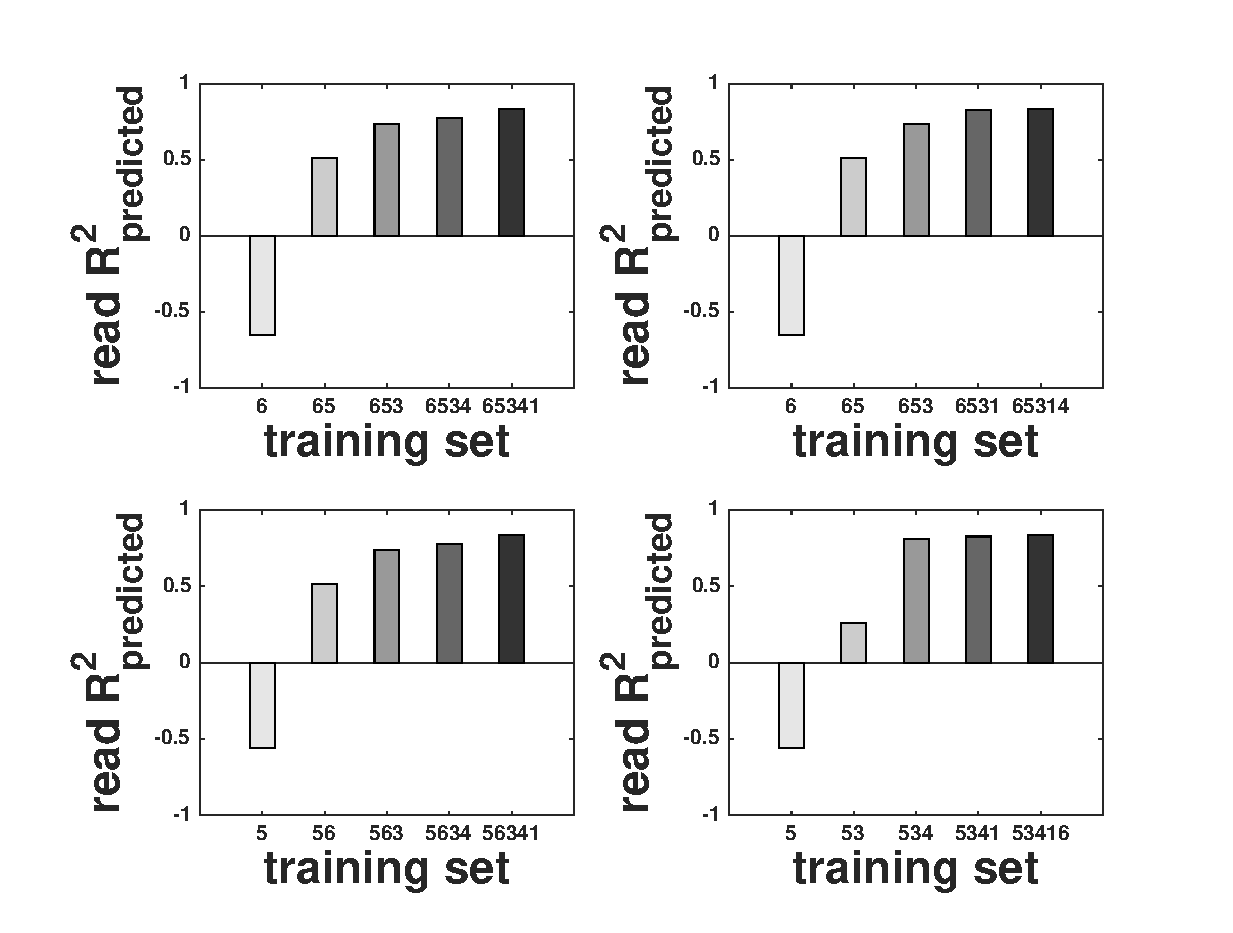
\includegraphics[scale = 0.4]{bar_read_avg_latency.eps}
  \end{figure}
\end{frame}

\begin{frame}
\frametitle{Redis}
  \begin{figure}
    \centering
    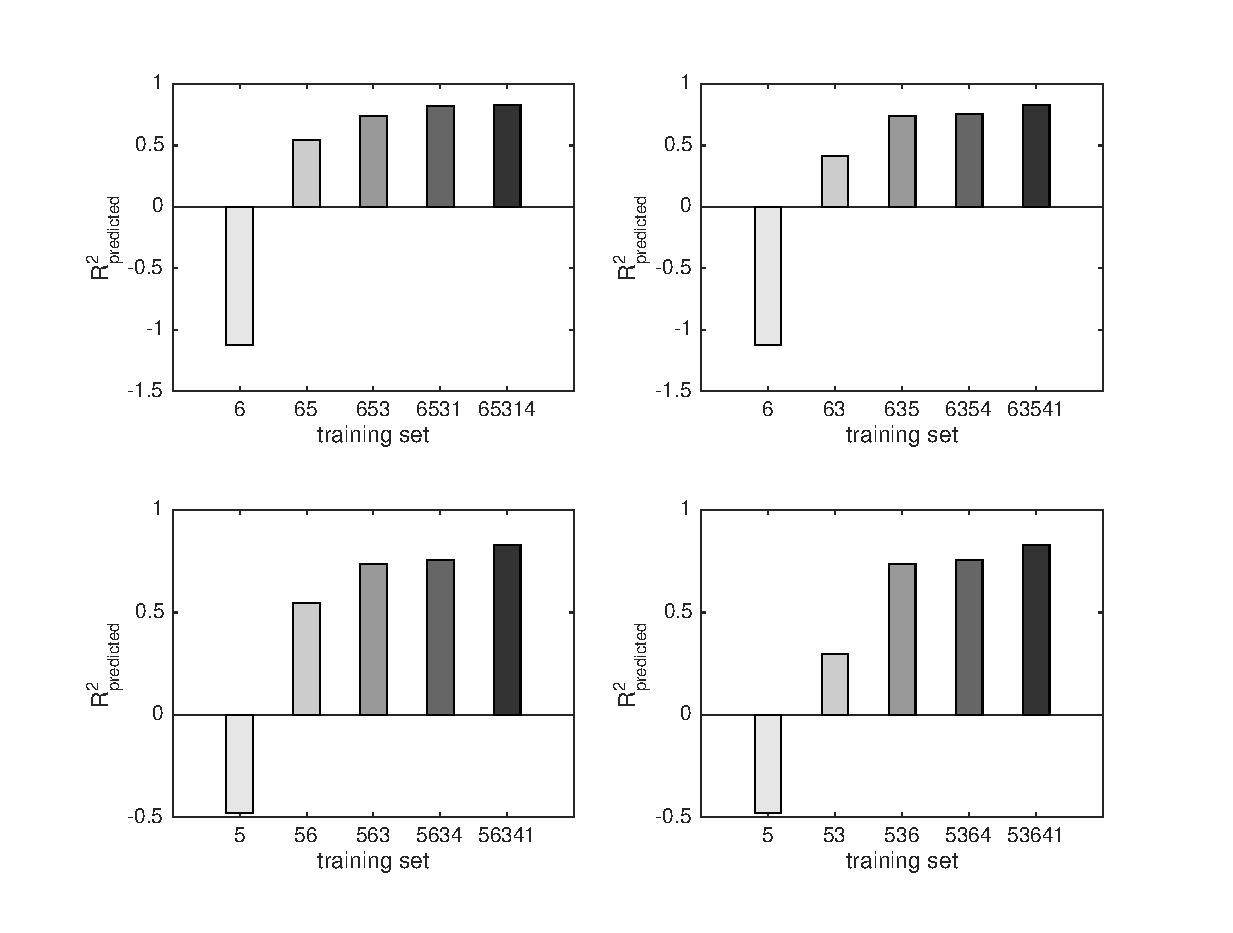
\includegraphics[scale = 0.4]{bar_write_avg_latency.eps}
  \end{figure}
\end{frame}

\begin{frame}
\frametitle{Redis}
\begin{figure}
\begin{tabular}{cc}
 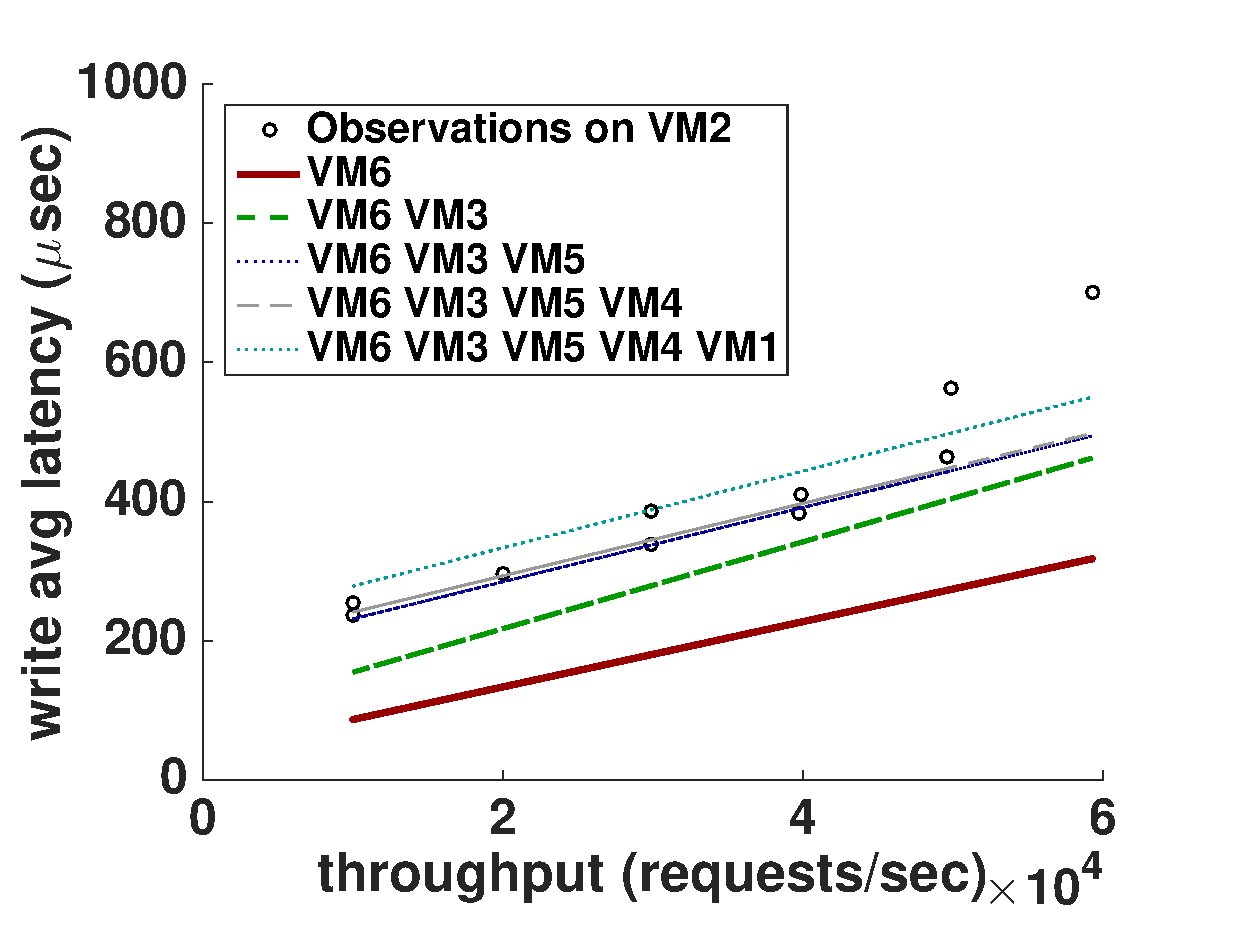
\includegraphics[width=0.35\textwidth]{fit_write_avg_latency_r3_2x_m3_2x_r3_x_r3__m3__m3_x.eps} &
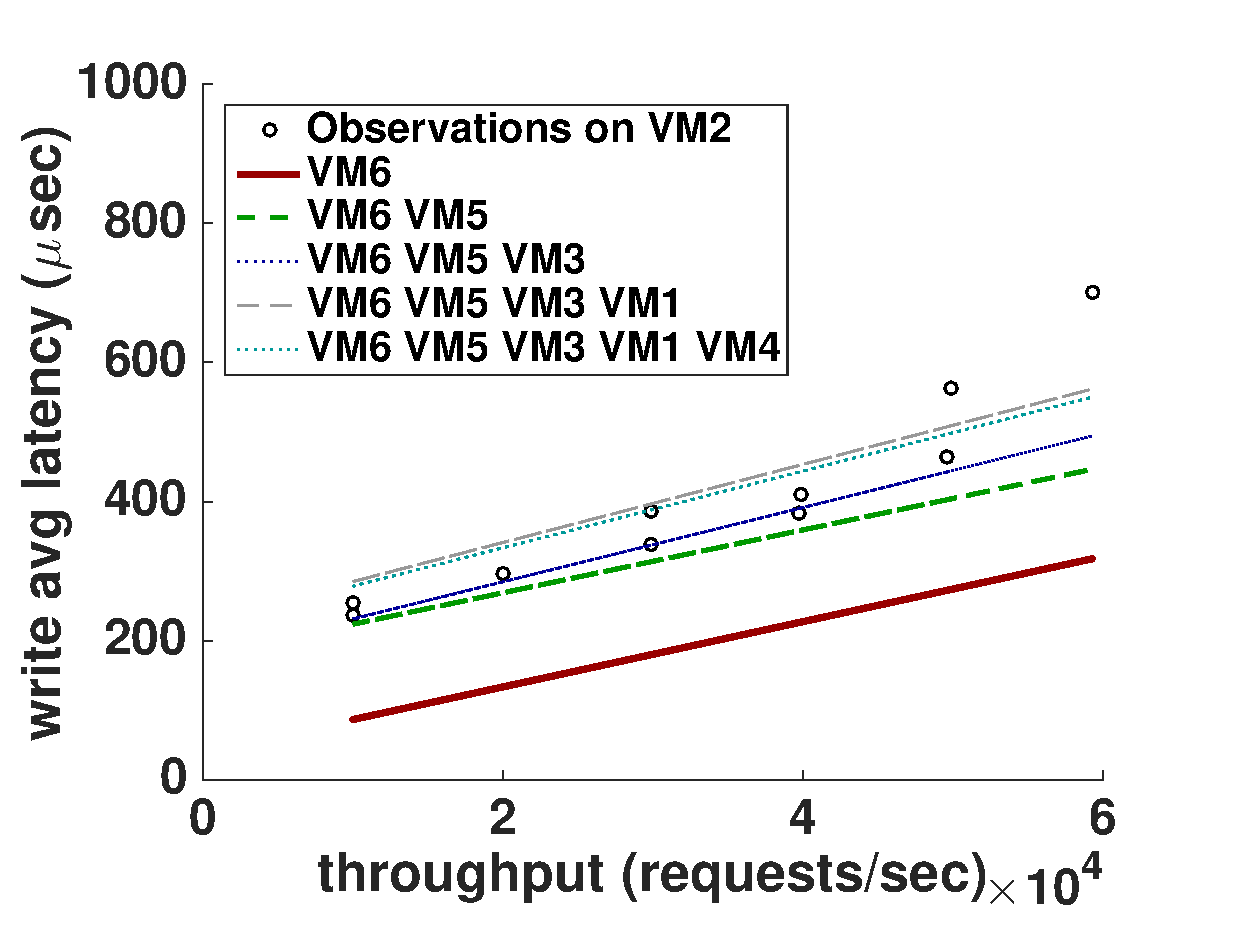
\includegraphics[width=0.35\textwidth]{fit_write_avg_latency_r3_2x_r3_x_m3_2x_m3__r3__m3_x.eps} \\
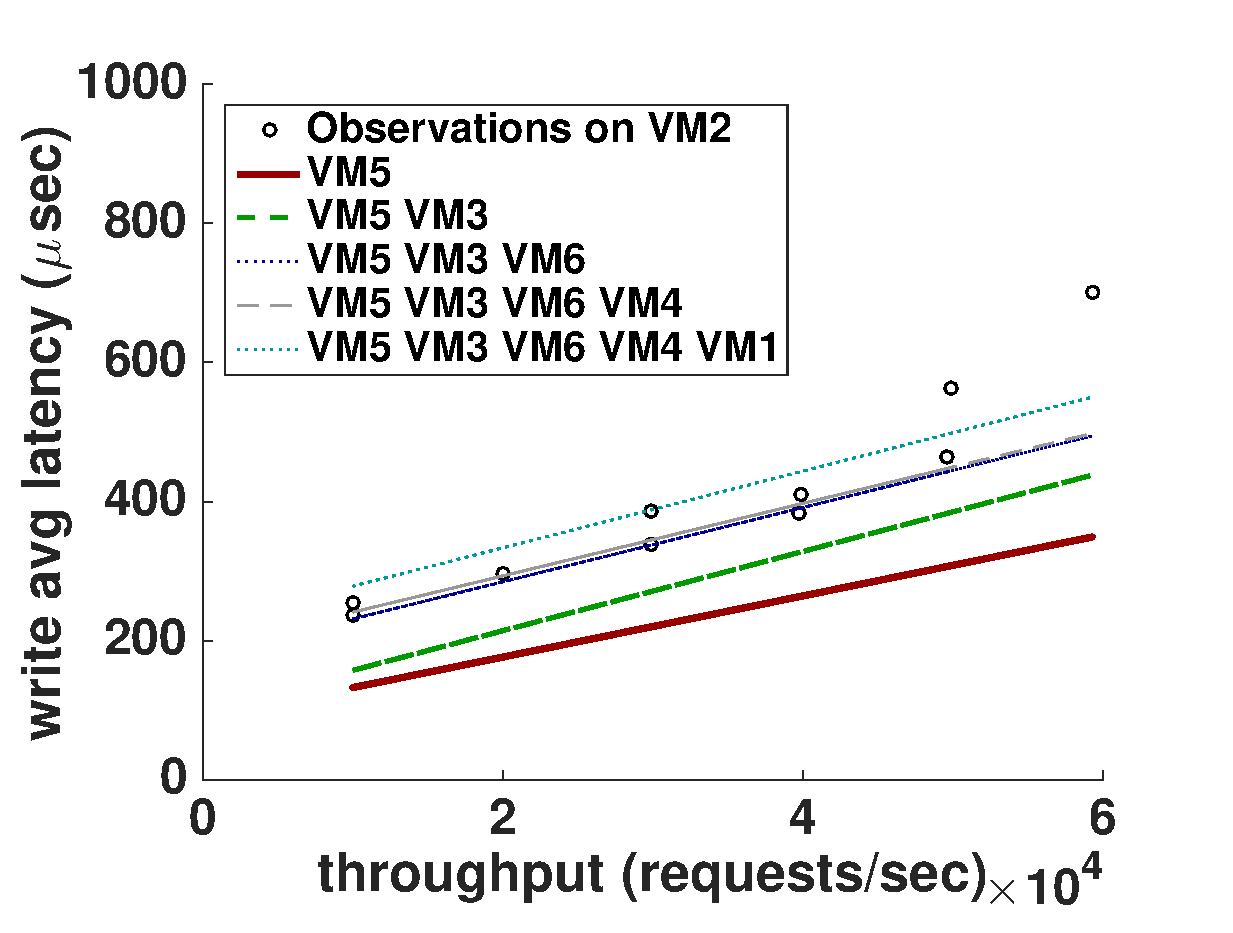
\includegraphics[width=0.35\textwidth]{fit_write_avg_latency_r3_x_m3_2x_r3_2x_r3__m3__m3_x.eps} &
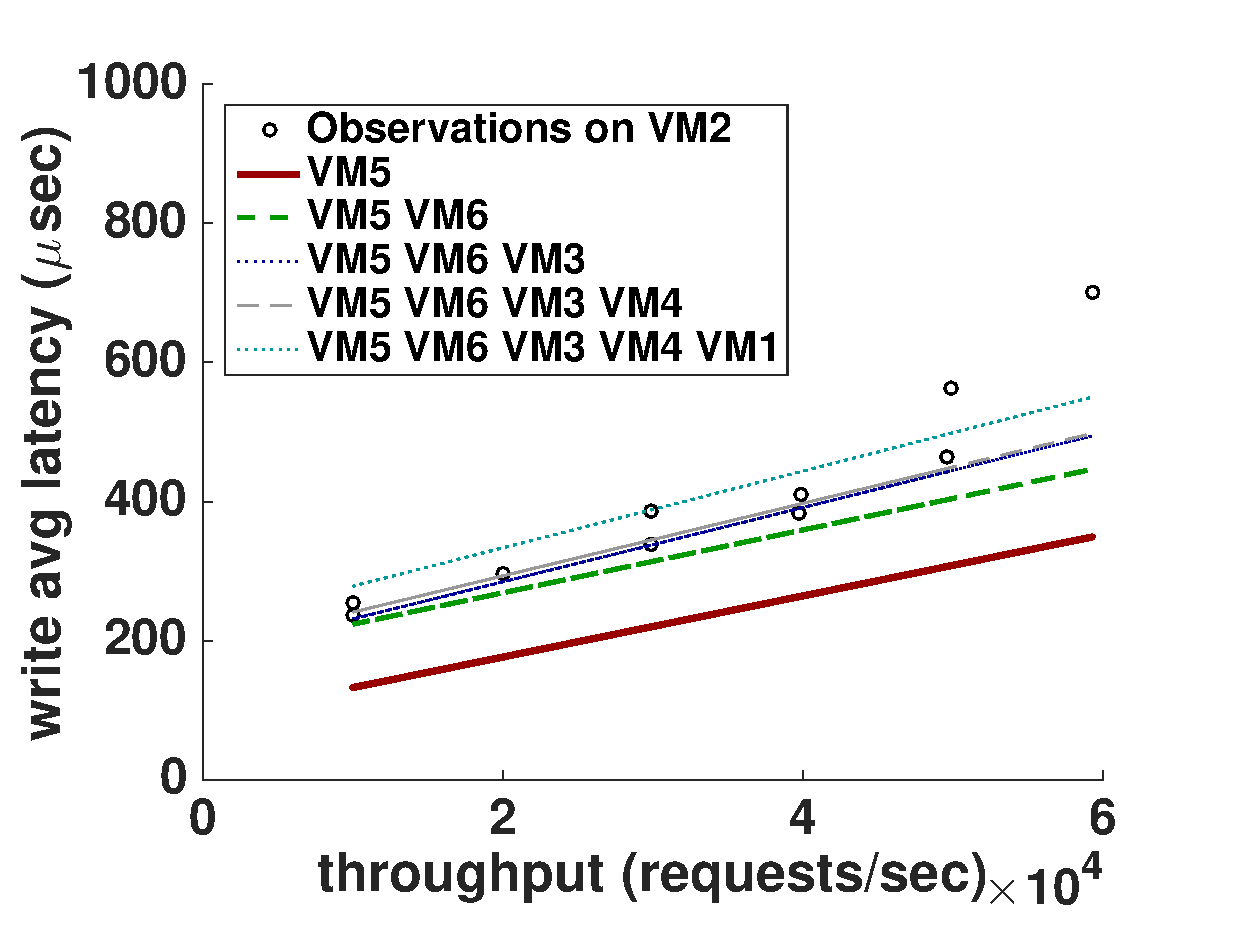
\includegraphics[width=0.35\textwidth]{fit_write_avg_latency_r3_x_r3_2x_m3_2x_r3__m3__m3_x.eps} \\ 
\end{tabular}
\caption{Prediction of Redis write latency on $VM_2$ compared for model calibration using a variety of training sets ranging in size from 1 to 5 VM types.}
\end{figure}
\end{frame}

\begin{frame}
\frametitle{Apache Cassandra: Table/Key-Value hybrid NoSQL database}
\begin{enumerate}
\item high availability provided by replication
\item Cassandra prioritizes availability and performance over consistency \begin{figure}[htbp]
\centering
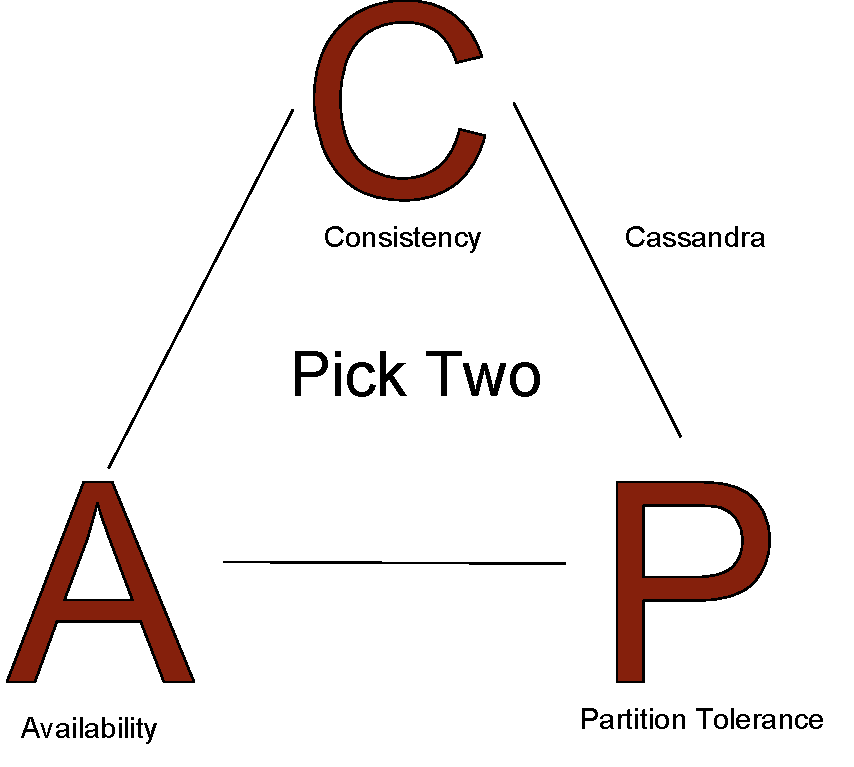
\includegraphics[width=0.4\textwidth]{CAP_diagram.pdf}
\end{figure}
\end{enumerate}
\end{frame}

\begin{frame}
\frametitle{Apache Cassandra: Table/Key-Value hybrid NoSQL database}
\begin{enumerate}
\item Cassandra clusters with 5 nodes
\item replication factor of three
\item consistency level of ONE (weak/eventual consistency)
\end{enumerate}
\end{frame}

\begin{frame}
\frametitle{Apache Cassandra}
  \begin{figure}
    \centering
    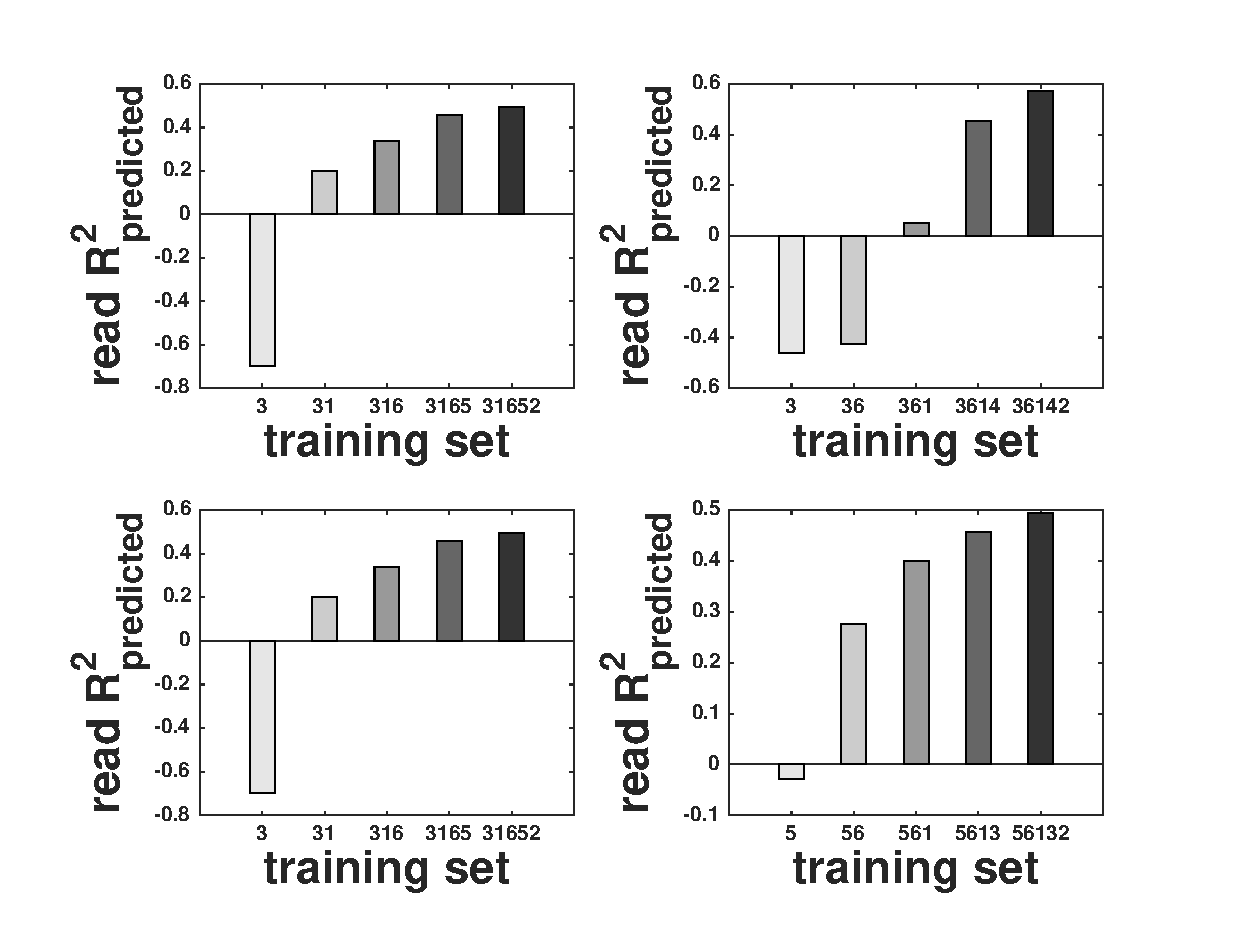
\includegraphics[scale = 0.4]{cassandra_bar_read_avg_latency.eps}
  \end{figure}
\end{frame}

\begin{frame}
\frametitle{Apache Cassandra}
  \begin{figure}
    \centering
    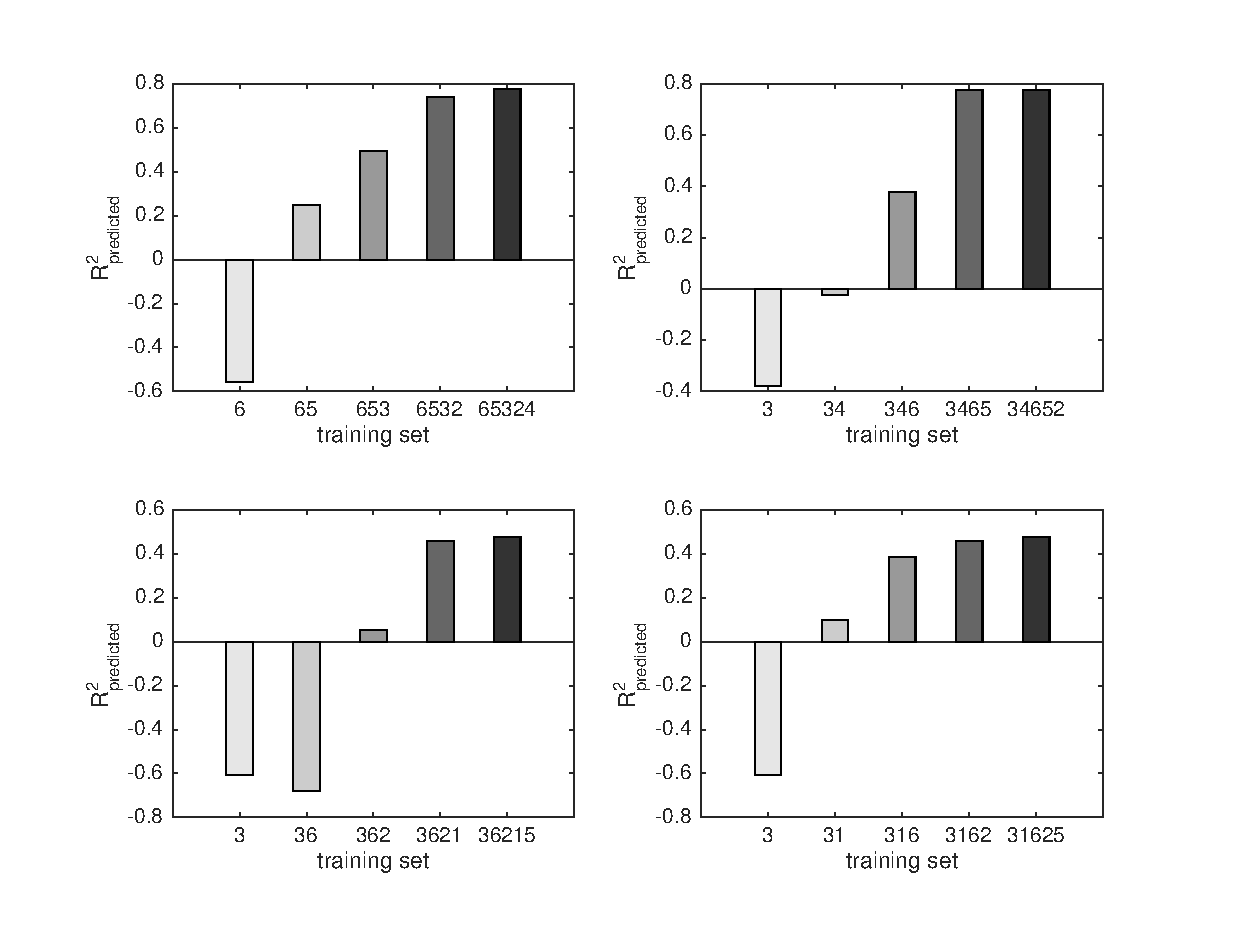
\includegraphics[scale = 0.4]{cassandra_bar_write_avg_latency.eps}
  \end{figure}
\end{frame}

\begin{frame}
\frametitle{Apache Cassandra}
\begin{figure}
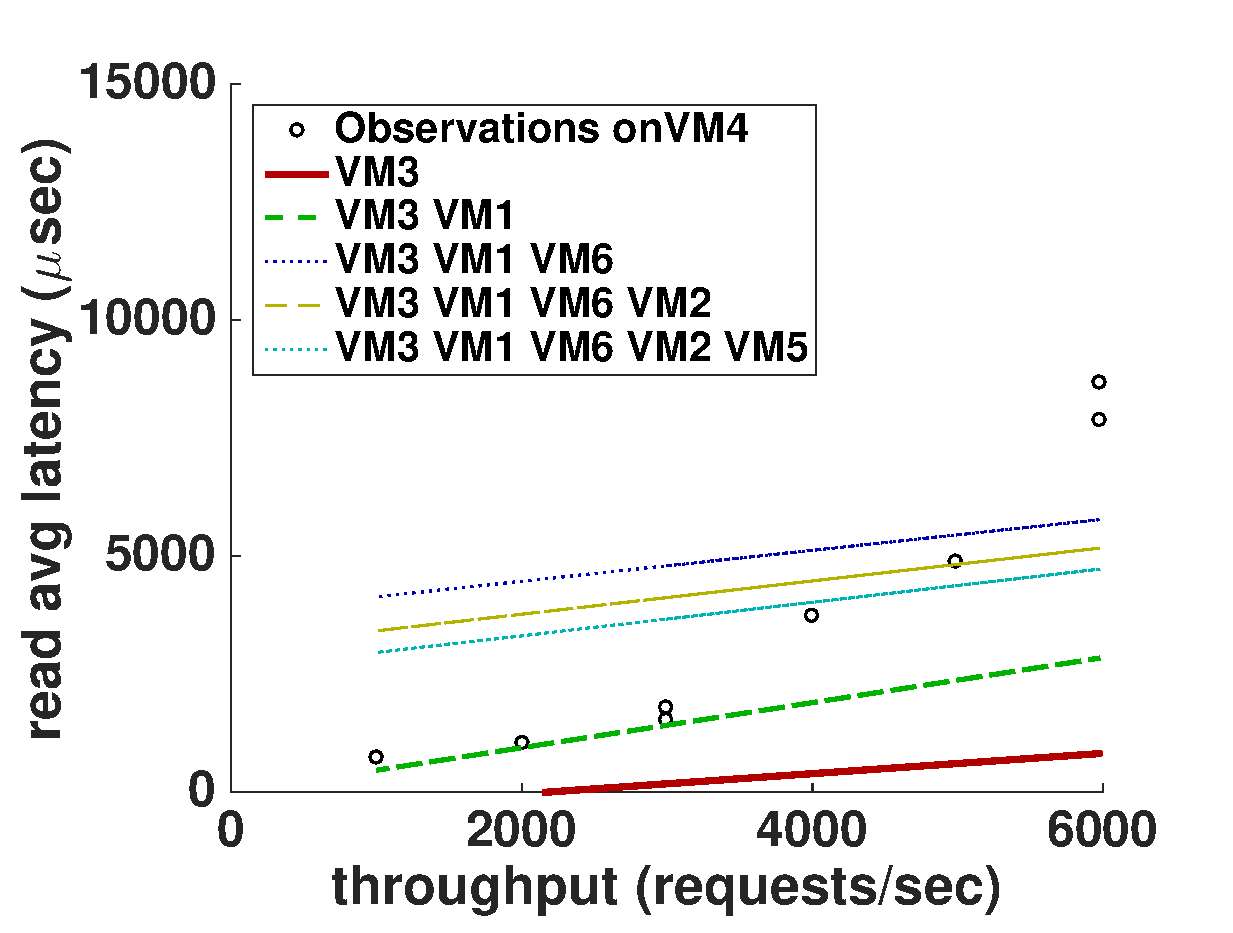
\includegraphics[width=0.25\textwidth]{cassandra_fit_read_avg_latency_m3_2x_m3__r3_2x_m3_x_r3_x_r3_.eps}
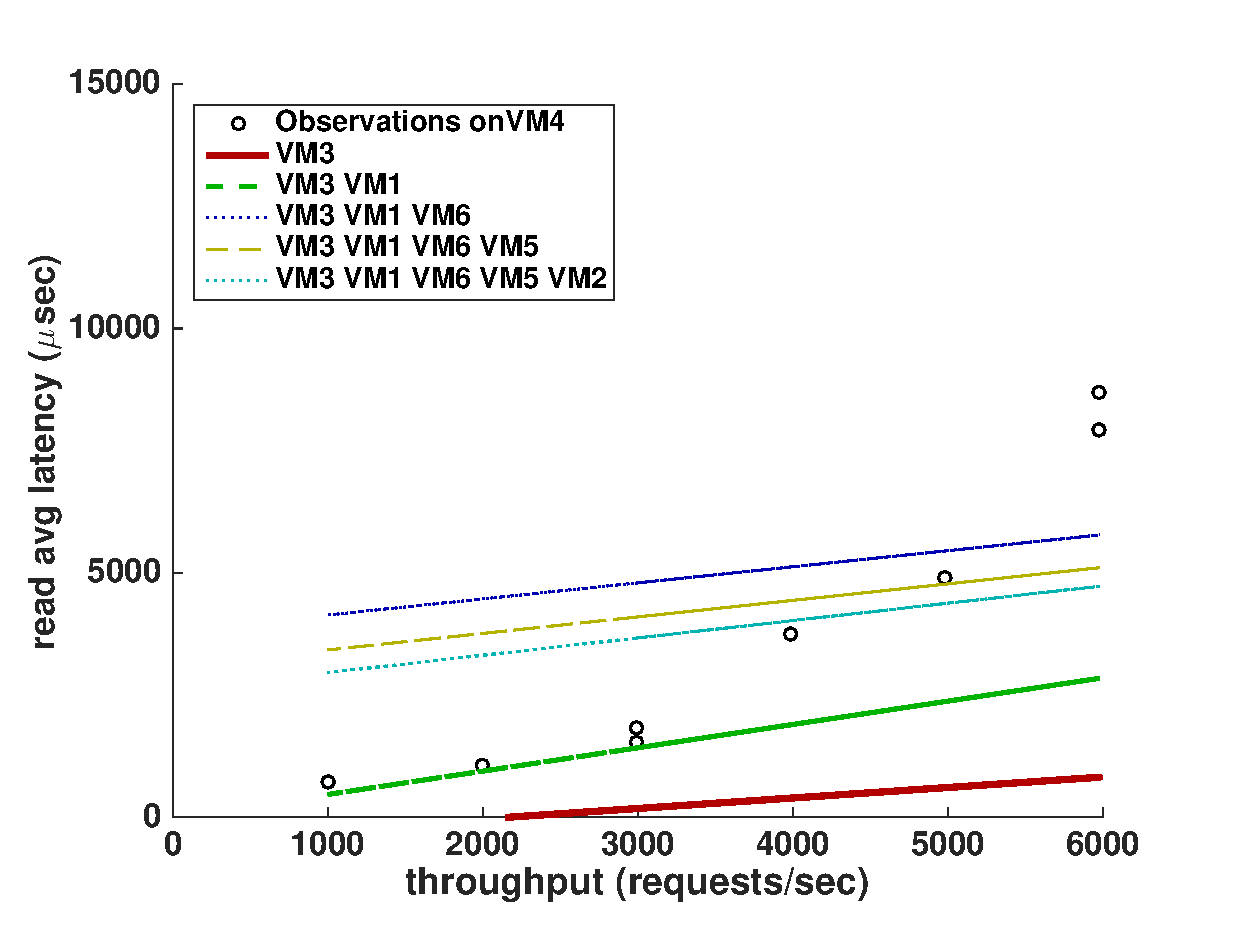
\includegraphics[width=0.25\textwidth]{cassandra_fit_read_avg_latency_m3_2x_m3__r3_2x_r3_x_m3_x_r3_.eps}
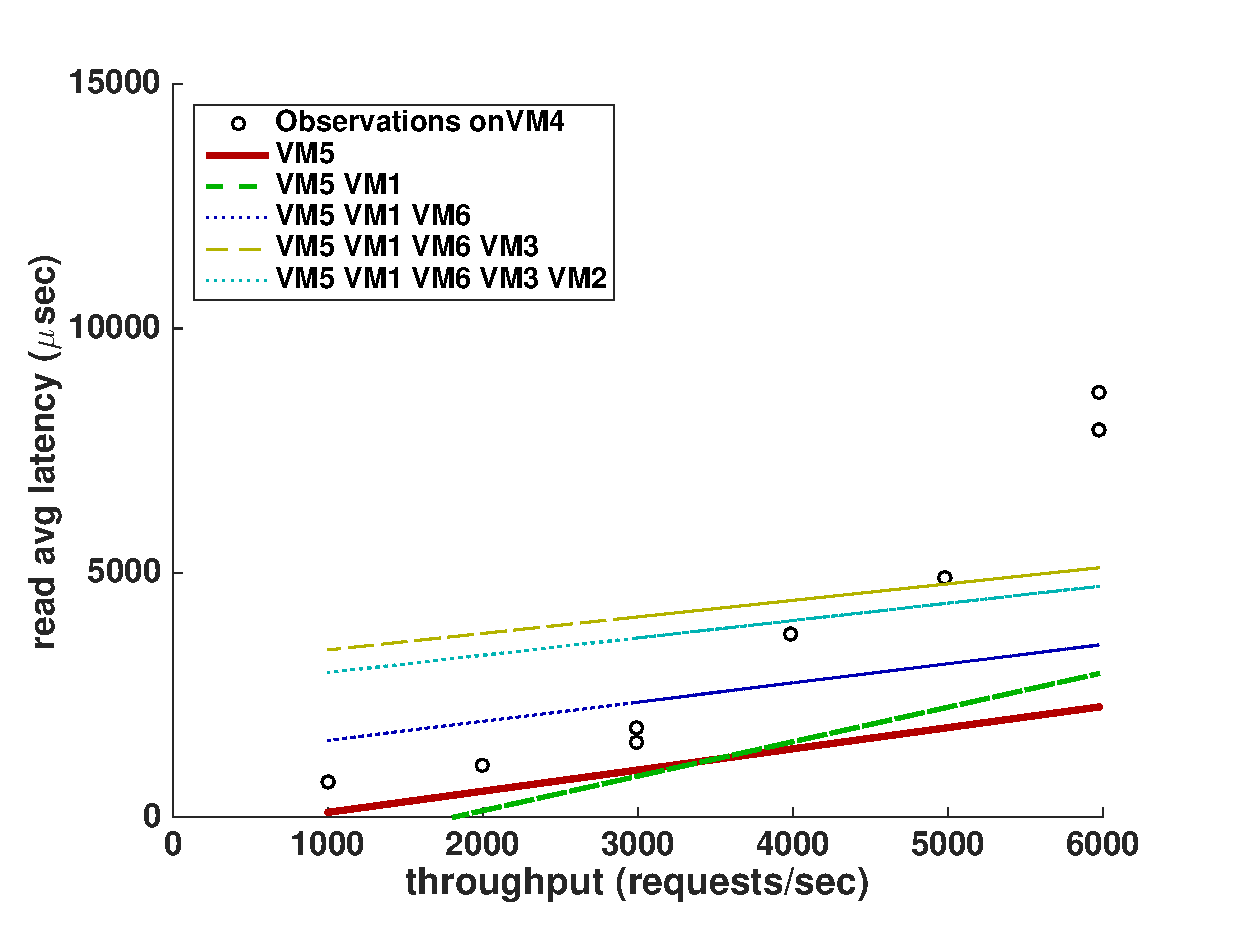
\includegraphics[width=0.25\textwidth]{cassandra_fit_read_avg_latency_r3_x_m3__r3_2x_m3_2x_m3_x_r3_.eps}
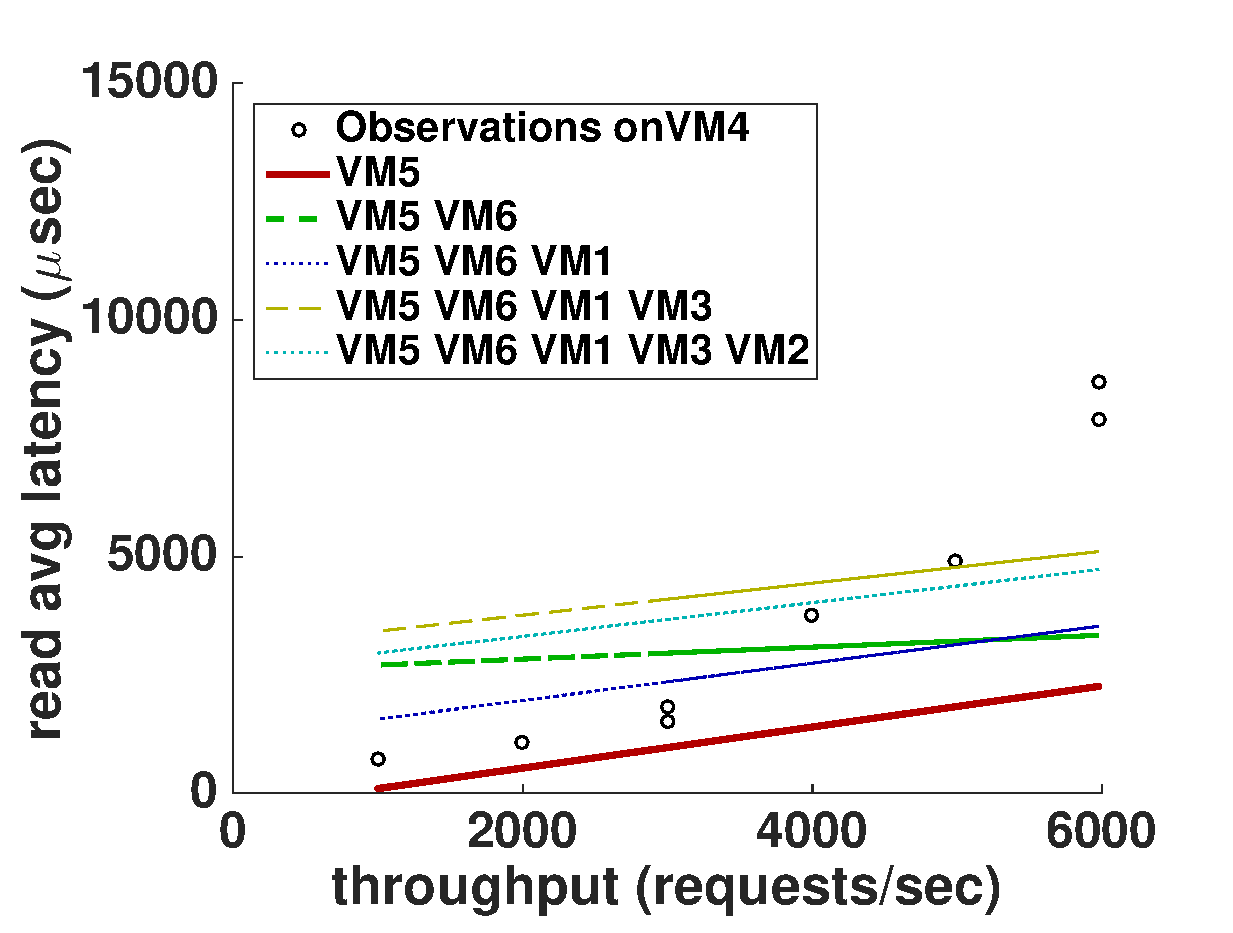
\includegraphics[width=0.25\textwidth]{cassandra_fit_read_avg_latency_r3_x_r3_2x_m3__m3_2x_m3_x_r3_.eps}
\caption{Prediction of Cassandra read latency on $VM_4$ compared for model calibration using a variety of training sets ranging in size from 1 to 5 VM types.}
\end{figure}
\end{frame}

\begin{frame}
\frametitle{Apache Cassandra}
\begin{figure}
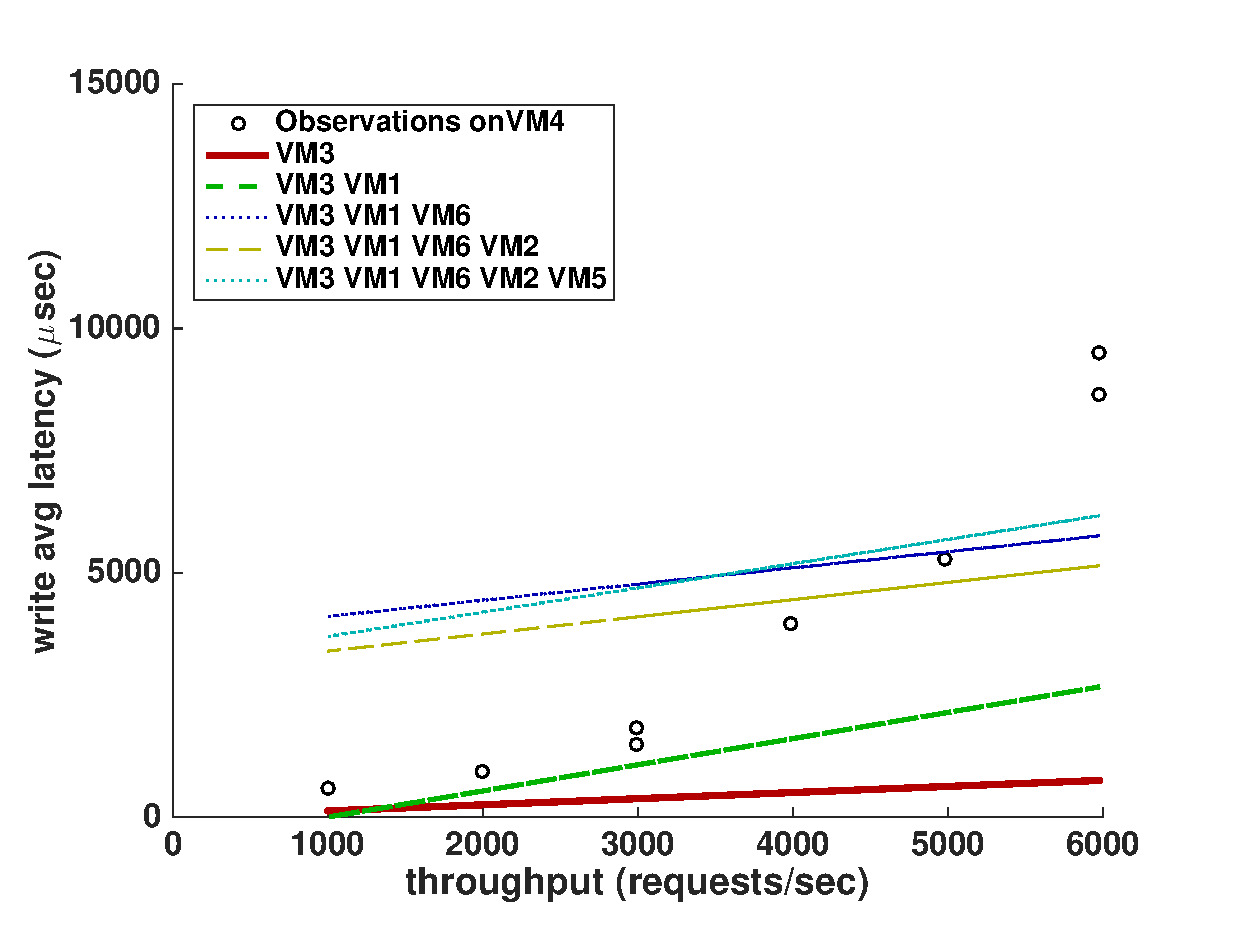
\includegraphics[width=0.25\textwidth]{cassandra_fit_write_avg_latency_m3_2x_m3__r3_2x_m3_x_r3_x_r3_.eps}
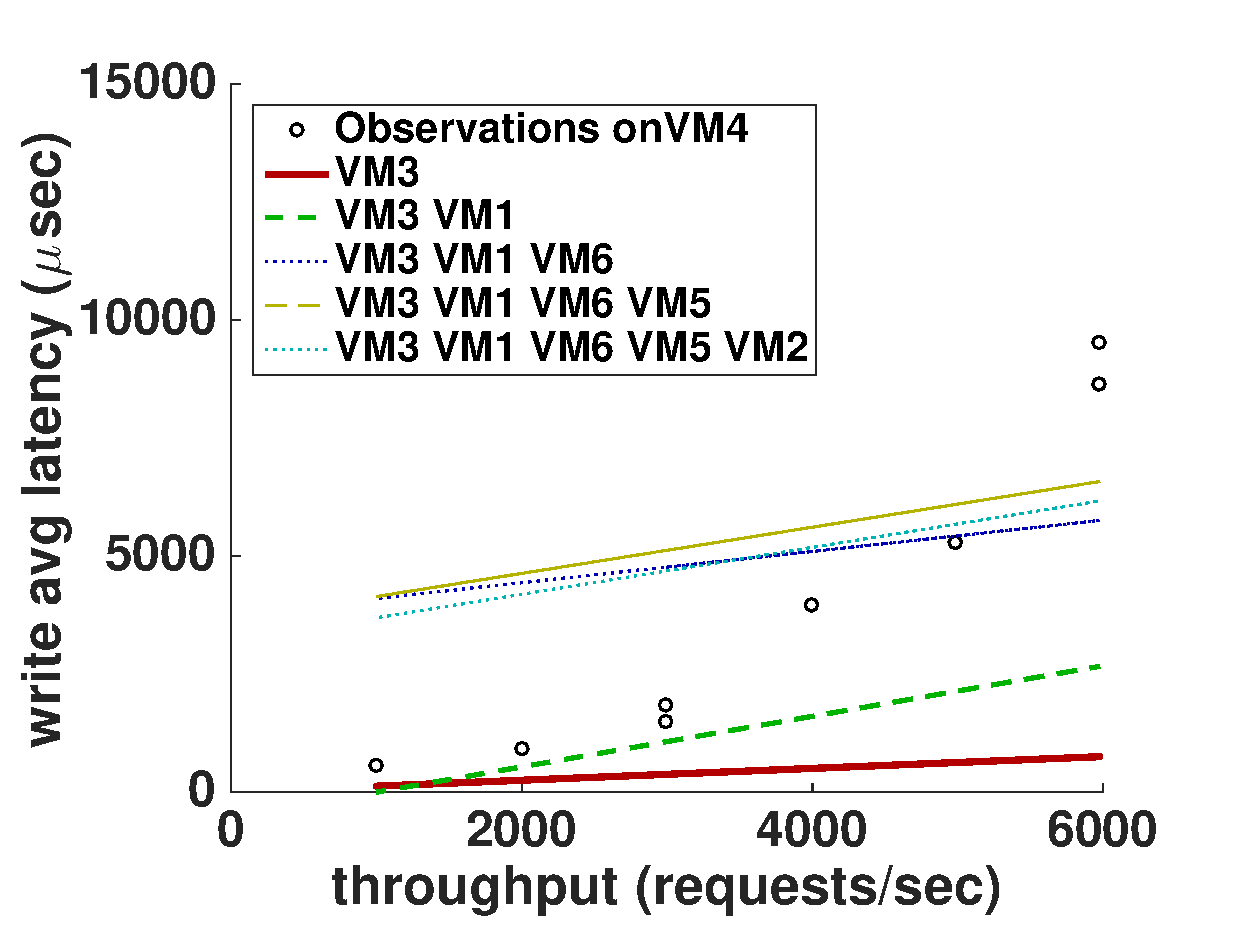
\includegraphics[width=0.25\textwidth]{cassandra_fit_write_avg_latency_m3_2x_m3__r3_2x_r3_x_m3_x_r3_.eps}
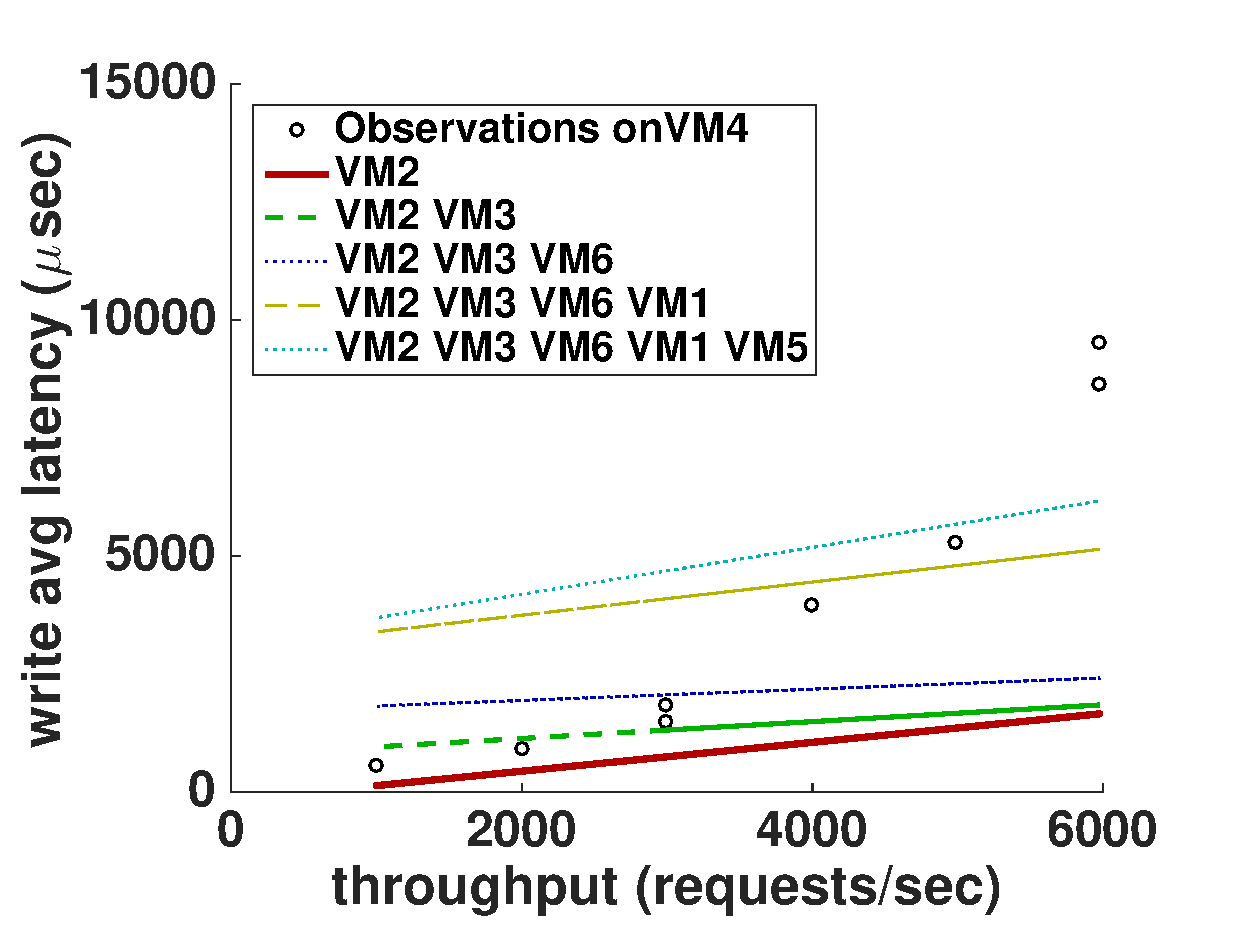
\includegraphics[width=0.25\textwidth]{cassandra_fit_write_avg_latency_m3_x_m3_2x_r3_2x_m3__r3_x_r3_.eps}
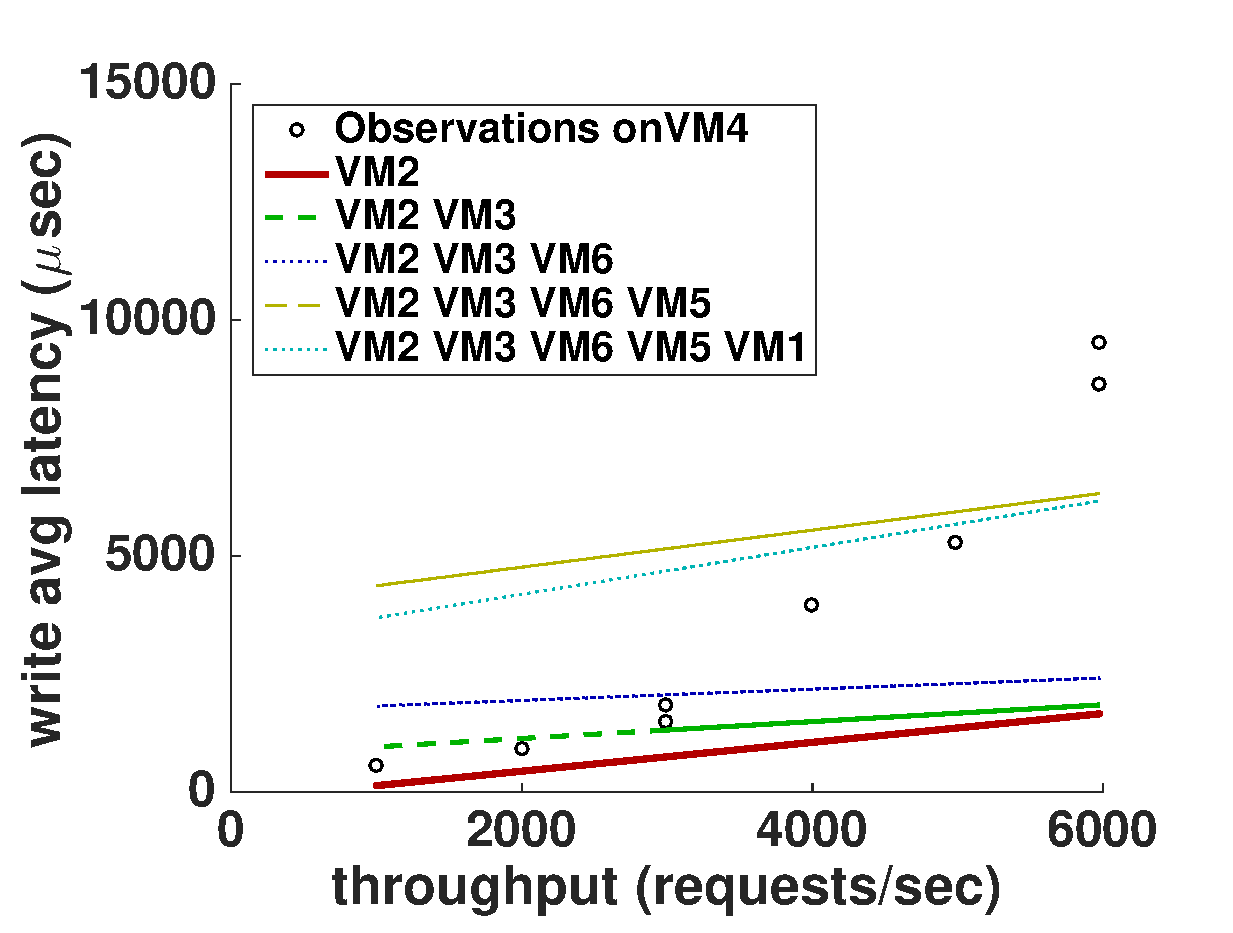
\includegraphics[width=0.25\textwidth]{cassandra_fit_write_avg_latency_m3_x_m3_2x_r3_2x_r3_x_m3__r3_.eps}
\caption{Prediction of Cassandra write latency on $VM_4$ compared for model calibration using a variety of training sets ranging in size from 1 to 5 VM types.}
\end{figure}
\end{frame}

\begin{frame}
\frametitle{MySQL}
\begin{enumerate}
\item RDBMS database
\item deployed with Amazon RDS
\end{enumerate}
\end{frame}

\begin{frame}
\frametitle{MySQL}
  \begin{figure}
    \centering
    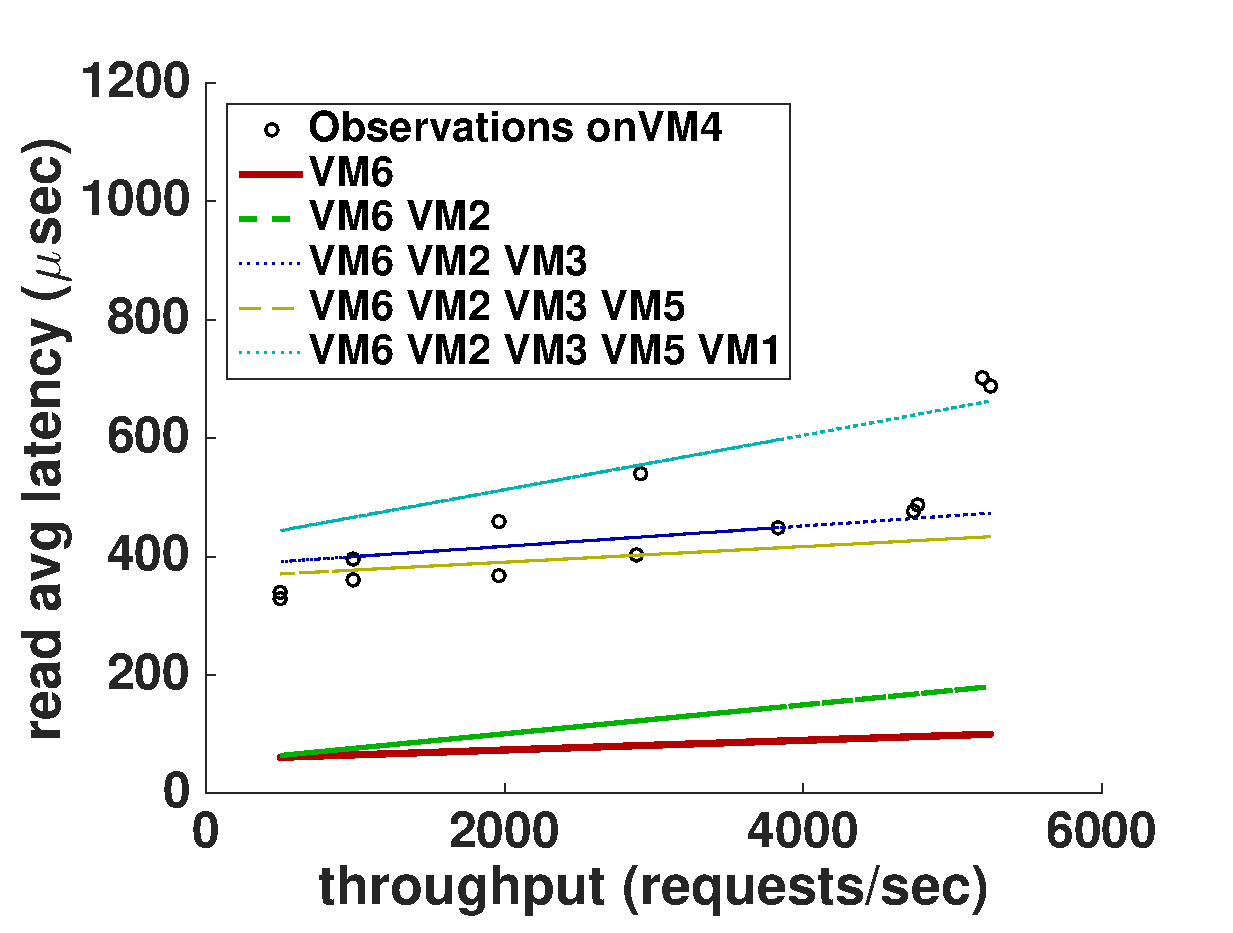
\includegraphics[scale = 0.3]{mysql_fit_read_avg_latency.eps}
    \caption{Read latency/throughput plot for MySQL; multiple linear regression model does not fit as well for MySQL compared to other case studies}
    \label{figure:mysql}
  \end{figure}
\end{frame}

\section{Conclusions}

\begin{frame}
\frametitle{Conclusions}
\begin{block}{Diversity of VM instance types}
Opportunity for black box data modeling with multiple linear regression
\end{block}
\begin{block}{Tested Latency vs. Throughput for 3 common database applications}
Redis, Cassandra, MySQL
\end{block}
\begin{block}{Found Model Accuracy improved with larger training sets}
With larger dataset, possibility of more accurately predicting performance for new VM instance types
\end{block}
\end{frame}

%------------------------------------------------
\begin{comment}
\begin{frame}
\frametitle{Bullet Points}
\begin{itemize}
\item Lorem ipsum dolor sit amet, consectetur adipiscing elit
\item Aliquam blandit faucibus nisi, sit amet dapibus enim tempus eu
\item Nulla commodo, erat quis gravida posuere, elit lacus lobortis est, quis porttitor odio mauris at libero
\item Nam cursus est eget velit posuere pellentesque
\item Vestibulum faucibus velit a augue condimentum quis convallis nulla gravida
\end{itemize}
\end{frame}

%------------------------------------------------

\begin{frame}
\frametitle{Blocks of Highlighted Text}
\begin{block}{Block 1}
Lorem ipsum dolor sit amet, consectetur adipiscing elit. Integer lectus nisl, ultricies in feugiat rutrum, porttitor sit amet augue. Aliquam ut tortor mauris. Sed volutpat ante purus, quis accumsan dolor.
\end{block}

\begin{block}{Block 2}
Pellentesque sed tellus purus. Class aptent taciti sociosqu ad litora torquent per conubia nostra, per inceptos himenaeos. Vestibulum quis magna at risus dictum tempor eu vitae velit.
\end{block}

\begin{block}{Block 3}
Suspendisse tincidunt sagittis gravida. Curabitur condimentum, enim sed venenatis rutrum, ipsum neque consectetur orci, sed blandit justo nisi ac lacus.
\end{block}
\end{frame}

%------------------------------------------------

\begin{frame}
\frametitle{Multiple Columns}
\begin{columns}[c] % The "c" option specifies centered vertical alignment while the "t" option is used for top vertical alignment

\column{.45\textwidth} % Left column and width
\textbf{Heading}
\begin{enumerate}
\item Statement
\item Explanation
\item Example
\end{enumerate}

\column{.5\textwidth} % Right column and width
Lorem ipsum dolor sit amet, consectetur adipiscing elit. Integer lectus nisl, ultricies in feugiat rutrum, porttitor sit amet augue. Aliquam ut tortor mauris. Sed volutpat ante purus, quis accumsan dolor.

\end{columns}
\end{frame}

%------------------------------------------------
%\section{Second Section}
%------------------------------------------------

\begin{frame}
\frametitle{Table}
\begin{table}
\begin{tabular}{l l l}
\toprule
\textbf{Treatments} & \textbf{Response 1} & \textbf{Response 2}\\
\midrule
Treatment 1 & 0.0003262 & 0.562 \\
Treatment 2 & 0.0015681 & 0.910 \\
Treatment 3 & 0.0009271 & 0.296 \\
\bottomrule
\end{tabular}
\caption{Table caption}
\end{table}
\end{frame}

%------------------------------------------------

\begin{frame}
\frametitle{Theorem}
\begin{theorem}[Mass--energy equivalence]
$E = mc^2$
\end{theorem}
\end{frame}

%------------------------------------------------

\begin{frame}[fragile] % Need to use the fragile option when verbatim is used in the slide
\frametitle{Verbatim}
\begin{example}[Theorem Slide Code]
\begin{verbatim}
\begin{frame}
\frametitle{Theorem}
\begin{theorem}[Mass--energy equivalence]
$E = mc^2$
\end{theorem}
\end{frame}\end{verbatim}
\end{example}
\end{frame}

%------------------------------------------------

\begin{frame}
\frametitle{Figure}
Uncomment the code on this slide to include your own image from the same directory as the template .TeX file.
%\begin{figure}
%\includegraphics[width=0.8\linewidth]{test}
%\end{figure}
\end{frame}

%------------------------------------------------

\begin{frame}[fragile] % Need to use the fragile option when verbatim is used in the slide
\frametitle{Citation}
An example of the \verb|\cite| command to cite within the presentation:\\~

This statement requires citation \cite{p1}.
\end{frame}

%------------------------------------------------

\begin{frame}
\frametitle{References}
\footnotesize{
\begin{thebibliography}{99} % Beamer does not support BibTeX so references must be inserted manually as below
\bibitem[Smith, 2012]{p1} John Smith (2012)
\newblock Title of the publication
\newblock \emph{Journal Name} 12(3), 45 -- 678.
\end{thebibliography}
}
\end{frame}
\end{comment}

%------------------------------------------------

\begin{frame}
\Huge{\centerline{The End}}
\end{frame}

%----------------------------------------------------------------------------------------
\end{document}